%-*- coding:utf-8 -*-

\documentclass[dvipdfmx]{beamer}
\usepackage{tutorial}

\title{計算機実験II (L4) --- 最適化}
\date{2018/12/21}

\begin{document}

\begin{frame}
  \titlepage
  \tableofcontents
\end{frame}

\section{最適化問題}

\begin{frame}[t,fragile]{最適化問題}
  \begin{itemize}
    \setlength{\itemsep}{1em}
  \item 目的関数$f(x)$の最小値(あるいは最大値)とその場所を求めたい
  \item どういう問題を解くのに使えるか?
    \begin{itemize}
    \item 変分原理が成り立つ問題: 最小作用の原理、最小エネルギーの原理
    \item コスト関数が定義できる問題: 最小二乗法(線形回帰、非線形回帰)、(連立)方程式の求階、機械学習
    \end{itemize}
  \item ほとんど全ての問題はコスト関数をうまく定義することで、最適化問題に書き換えることができる
    \begin{itemize}
    \item (一般に)最適化問題として解くのは最終手段
    \item もっと良い方法があるときはそちらを使う
    \end{itemize}
  \end{itemize}
\end{frame}

\begin{frame}[t,fragile]{最適化問題}
  \begin{itemize}
    %\setlength{\itemsep}{1em}
  \item 最適化問題の種類
    \begin{itemize}
    \item 連続最適化問題 $\Leftarrow$ 難しい
    \item 離散最適化(組み合わせ最適化)問題 $\Leftarrow$ もっと難しい
    \end{itemize}
  \item 真の(大局的な)最小値(最大値)を求めるのは難しい
  \item 一般的には極値を求めることしかできない
  \item 多次元では極小を囲い込むことができない
  \item 導関数を使う方法: ニュートン法、準ニュートン法、最急降下法、勾配降下法、共役勾配法$\cdots$
  \item 使わない方法: 囲い込み法、Nelder-Meadの滑降シンプレックス法、シミュレーテッド・アニーリング$\cdots$
  \item コスト関数・導関数の評価回数と収束までの反復回数のトレードオフ
  \end{itemize}
\end{frame}

\begin{frame}[t,fragile]{ニュートン法}
  \begin{itemize}
    \setlength{\itemsep}{1em}
  \item 反復法により方程式$f(x)=0$の解を求める
  \item 真の解を$x_0$、現在の解の候補を$x_n=x_0+\epsilon$とすると
    \[
    0 = f(x_0) = f(x_0+\epsilon-\epsilon) = f(x_n) - f'(x_n) \epsilon + O(\epsilon^2)
    \]
  \item 次の解の候補 (反復法、逐次近似法)
    \[
    \epsilon \approx \frac{f(x_n)}{f'(x_n)} \quad\quad x_{n+1} = x_n - \frac{f(x_n)}{f'(x_n)}
    \]
  \item 複素変数の複素関数や多変数の場合にも自然に拡張可
  \end{itemize}
\end{frame}

\begin{frame}[t,fragile]{多次元の場合}
  \begin{itemize}
    \setlength{\itemsep}{1em}
  \item $f(x)=0$: $d$次元(非線形)連立方程式
  \item $x$は$d$次元のベクトル: $x = {}^t(x_1,x_2,\cdots,x_d)$
  \item $f(x)$も$d$次元のベクトル: $f(x) = {}^t(f_1(x), f_2(x),\cdots,f_d(x))$
  \item 真の解のまわりでの展開 ($x_n = x_0 + \epsilon$)
    \[
    0 = f(x_0) = f(x_0+\epsilon-\epsilon) = f(x_n) - \frac{\partial f(x_n)}{\partial x} \cdot \epsilon + O(|\epsilon|^2)
    \]
  \item ヤコビ行列($d\times d$): $\displaystyle \Big[\frac{\partial f(x)}{\partial x}\Big]_{ij} = \frac{\partial f_i(x)}{\partial x_j}$
  \item 次の解の候補: $\displaystyle x_{n+1} = x_n - \Big[\frac{\partial f(x_n)}{\partial x}\Big]^{-1} f(x_n)$
  \end{itemize}
\end{frame}

\begin{frame}[t,fragile]{ニュートン法による最適化}
  \begin{itemize}
    \setlength{\itemsep}{1em}
  \item $x$は$d$次元のベクトル: $x = {}^t(x_1,x_2,\cdots,x_d)$、目的関数$f(x)$はスカラー
  \item 勾配ベクトル: $\displaystyle [\nabla f(x)]_i = \frac{\partial f(x)}{\partial x_i}$
  \item 極小値(最小値)となる条件: $\nabla f(x)=0$
  \item ニュートン法で$f(x)$を$\nabla f(x)$で置き換えればよい
  \item 次の解の候補: $\displaystyle x_{n+1} = x_n - H^{-1}(x_n) \nabla f(x_n)$
  \item ヘッセ行列(Hessian): $\displaystyle H_{ij}(x) = \frac{\partial^2 f}{\partial x_i \partial x_j}(x)$
  \end{itemize}
\end{frame}

\begin{frame}[t,fragile]{準ニュートン法}
  \begin{itemize}
    %\setlength{\itemsep}{1em}
  % \item ニュートン法では、ヘッセ行列の計算・保存が必要
  \item 準ニュートン法: それまでの反復で計算した勾配ベクトルから、ヘッセ行列の逆行列を近似($C_n \approx H^{-1}$)
  \begin{itemize}
    \item 極小点の近傍では
      \begin{align*}
          x-x_n &= -H^{-1} \cdot \nabla f(x_n) \\
          x-x_{n+1} &= -H^{-1} \cdot \nabla f(x_{n+1})
      \end{align*}
    \item 差をとると($s_n = x_{n+1} - x_n$, $y_n = \nabla f(x_{n+1}) - \nabla f(x_n)$)
      \begin{align*}
        s_n &= H^{-1} \cdot y_n
      \end{align*}
    \item この式が満たされるように、$C_{n+1}$を$C_{n}+(\text{補正})$の形で構成(DFP法: Davidon-Fletcher-Powell)
      \[
        C_{n+1} = C_{n} + \frac{s_n s_n^T}{s_n^T y_n} - \frac{C_{n} y_n (C_{n} y_n)^T}{y_n^T C_n y_n}
      \]
    \item 他にも、BFGS法など
    \end{itemize}
  \end{itemize}
\end{frame}

\input{7_optimization/enclosure.tex}
\section{最急降下法と勾配降下法}

\begin{frame}[t,fragile]{最急降下法(steepest descent)}
  \begin{itemize}
    \setlength{\itemsep}{1em}
  \item 関数の微分の情報を使う
  \item 現在の点$\bf x$における勾配を計算
    \[
    -\nabla f|_i = -\frac{\partial f}{\partial x_i}
    \]
  \item 坂を下る方向にそって、一次元最適化
  \item 動いた先の勾配の方向でさらに最適化を繰り返す
  \item 関数値は単調減少 $\Rightarrow$ 極小値に収束
  \end{itemize}
\end{frame}

\begin{frame}[t,fragile]{勾配降下法(gradient descent)}
  \begin{itemize}
    \setlength{\itemsep}{1em}
  \item 勾配方向に一次元最適化を行うかわりに、あらかじめ決めた一定量($\epsilon$)だけ坂を下る
    \[
    x_{n+1} = x_n - \epsilon \, \nabla f
    \]
  \item あらかじめ最適な$\epsilon$を知るのは困難
  \item 機械学習の分野では、(なぜか) $\epsilon=0.1$が良いとされている
  \item この方法を「最急降下法」、一次元最適化を行う勾配法を「最適降下法(optimum descent)」と呼ぶ場合も
  % \item c.f.) 確率的勾配降下法(stochastic gradient descent)
  \end{itemize}
\end{frame}

\begin{frame}[t,fragile]{制約条件付きの場合}
  \begin{itemize}
    % \setlength{\itemsep}{1em}
  \item 目的関数: $f(x)$
  \item 制約条件:
    \begin{itemize}
    \item $g_i(x) = 0$ \ ($i=1,\cdots,m$) \ (等式制約条件)
    \item $h_j(x) \ge 0$ \ ($j=1,\cdots,n$) \ (不等式制約条件)
    \end{itemize}
  \item 等式制約条件の付いている場合: Lagrangeの未定乗数法
    \[
    L(x,\lambda_1,\cdots,\lambda_m)=f(x)+\sum_i \lambda_i g_i(x)
    \]
    を考え、$x,\lambda_1,\cdots,\lambda_m$に関する微分が零となる点を探す
  \item 不等式制約条件の付いている場合: 線形計画法, ペナルティ関数法
  \end{itemize}
\end{frame}

\begin{frame}[t,fragile]{細長い谷の場合}
  \vspace*{1em}
  \hspace*{1em}\resizebox{1\textwidth}{!}{\includegraphics{image/steepest-descent.pdf}}

  \vspace*{-2em}
  \hspace*{20em}{\footnotesize(Press et al 1988)}
\end{frame}

\section{共役勾配法}

\begin{frame}[t,fragile]{共役勾配法(conjugate gradient)}
  \begin{itemize}
    \setlength{\itemsep}{1em}
  \item 目的関数がある点のまわりで
    \[
    f({\bf x}) \approx c - {\bf b}^T {\bf x} + \frac{1}{2} {\bf x}^T A {\bf x}
    \]
    と近似できるとする
  \item ${\bf x}$における勾配は、連立方程式$A{\bf x}={\bf b}$の「残差」の形で書ける
    \[
    -\nabla f = {\bf b} - A {\bf x}
    \]
  \item 新しい勾配方向ではなく、それまでとは「共役な方向」に進みたい
  \end{itemize}
\end{frame}

\begin{frame}[t,fragile]{「共役な方向」とは}
  \begin{itemize}
    \setlength{\itemsep}{1em}
  \item あるベクトル${\bf p}$にそった一次元の最適化が完了したとする
    \begin{itemize}
    \item その点における${\bf p}$方向の勾配は零。すなわち${\bf p}^T (\nabla f)=0$
    \item ${\bf p}$方向の勾配の値を変化させないようにしたい
  \end{itemize}
  \item 次に、${\bf q}$にそって、${\bf x}+\epsilon {\bf q}$と移動するとする。その時の勾配の変化は
    \[
      \delta(\nabla f) = A \times (\epsilon {\bf q}) \sim A {\bf q}
      \]
      これが${\bf p}$に垂直であるためには
    \[
      {\bf p}^T A {\bf q} = 0
      \]
    \item この関係が成り立つ時、${\bf p}$と${\bf q}$は「互いに共役」という
  \end{itemize}
\end{frame}

\begin{frame}[t,fragile]{共役勾配法(conjugate gradient)}
  \begin{itemize}
    \setlength{\itemsep}{1em}
  \item 初期条件: 位置 ${\bf x} = {\bf x}_0$
    \begin{align*}
      & \text{勾配:} \ {\bf p} = {\bf p}_0 = -\nabla f({\bf x}_0) = {\bf b} - A {\bf x}_0 \\
      & \text{残差:} \ {\bf r} = {\bf r}_0 = {\bf p}_0
    \end{align*}
  \item 最適化(第$n$ステップ)
    \begin{align*}
      \alpha_n &= \frac{{\bf r}_n^T {\bf p}_n}{{\bf p}_n^T A {\bf p}_n} \\
            {\bf x}_{n+1} &= {\bf x}_n + \alpha_n {\bf p}_n \\
            {\bf r}_{n+1} &= {\bf r}_n - \alpha_n A {\bf p}_n = {\bf b} - A {\bf x}_{n+1} \\
            \beta_n &= - \frac{{\bf p}_{n}^T A {\bf r}_{n+1}}{{\bf p}_n^T A {\bf p}_n} \\
                 {\bf p}_{n+1} &= {\bf r}_{n+1} + \beta_n {\bf p}_n
    \end{align*}
  \end{itemize}
\end{frame}

\begin{frame}[t,fragile]{共役勾配法 - 直線上の最適化}
  \begin{itemize}
    \setlength{\itemsep}{1em}
  \item 直線${\bf x} = {\bf x}_n + \alpha {\bf p}_n$上での最適化
  \item 点${\bf x}$で$f({\bf x})$が最小値をとるためには、${\bf x}$における勾配と直線の方向ベクトル${\bf p_n}$が垂直にならなければならない
    \begin{align*}
      -[\nabla f({\bf x})]^T {\bf p}_n &= ({\bf b} - A {\bf x})^T {\bf p}_n = {\bf r}^T {\bf p}_n = ({\bf b} - A ({\bf x}_n+\alpha {\bf p}_n))^T {\bf p}_n \\ &= ({\bf r}_n - \alpha A {\bf p}_n)^T {\bf p}_n = 0
    \end{align*}
    (${\bf r}_n \equiv {\bf b} - A{\bf x}_ n$)
  \item 最適解: $\displaystyle \alpha = \frac{{\bf r}_n^T {\bf p}_n}{{\bf p}_n^T A {\bf p}_n}$
  \end{itemize}
\end{frame}

\begin{frame}[t,fragile]{共役勾配法 - 共役な方向の決め方}
  \begin{itemize}
    \setlength{\itemsep}{1em}
  \item 新たな最適化方向: ${\bf p}_{n+1} = {\bf r}_{n+1} + \beta_n {\bf p}_n$
  \item $\beta_n=0$とすると最急降下法と等価
  \item 共役勾配法では、${\bf p}_{n+1}$と${\bf p}_{n}$が共役となるように$\beta_n {\bf p}_n$だけ補正を加える
    \begin{align*}
      {\bf p}_n^T A {\bf p}_{n+1} = {\bf p}_n^T A ({\bf r}_{n+1} + \beta_n {\bf p}_n) = 0
    \end{align*}
  \item $\beta_n$について解くと
    \begin{align*}
      \beta_n &= - \frac{{\bf p}_{n}^T A {\bf r}_{n+1}}{{\bf p}_n^T A {\bf p}_n}
    \end{align*}
  \end{itemize}
\end{frame}

\begin{frame}[t,fragile]{共役勾配法 - 共役性と直交性}
  \begin{itemize}
    \setlength{\itemsep}{1em}
  \item 共役性: $\{{\bf p}_i\}$は自動的に互いに共役となる
    \begin{align*}
      {\bf p}_i^T A {\bf p}_j &= 0 \qquad \text{($i < j \le n$)}
    \end{align*}
  \item ${\bf x}_n$を通り${\bf p}_0 \cdots {\bf p}_n$に並行な「平面」上で$f({\bf x}_{n+1})$は最小
    \begin{align*}
      {\bf p}_i^T {\bf r}_{n+1} &= 0 \qquad \text{($i \le n$)}
    \end{align*}
  \item 直交性: $\{{\bf r}_i\}$は自動的に互いに直交する
    \begin{align*}
      {\bf r}_i^T {\bf r}_j &= 0 \qquad \text{($i < j \le n+1$)}
    \end{align*}
  \item $N$回反復すると残差は零 (実際は数値誤差により直交性がくずれる)
  \end{itemize}
\end{frame}

\begin{frame}[t,fragile]{共役勾配法による連立一次方程式の求階}
  \begin{itemize}
    %\setlength{\itemsep}{1em}
  \item 行列$A$を正定値対称行列とする
  \item 連立方程式$A{\bf x}={\bf b}$の解を$\hat{\bf x}$とすると、目的関数
    \begin{align*}
      f({\bf x}) = \frac{1}{2} (\hat{\bf x} - {\bf x})^T A (\hat{\bf x} - {\bf x})
    \end{align*}
    は${\bf x} = \hat{\bf x}$の時、最小値0をとる
  \item ${\bf x}$における目的関数の勾配は、連立方程式の「残差」の形で書ける
    \begin{align*}
      -\nabla f = A (\hat{\bf x} - {\bf x}) = {\bf b} - A {\bf x} \equiv {\bf r}
    \end{align*}
  \item $f({\bf x})$の値を計算するには真の解$\hat{\bf x}$が必要だが、$f({\bf x})$の値そのものではなく勾配のみがあれば良い
  \item 行列ベクトル積だけで計算できるので、$A$が疎行列の時、特に有効
  \end{itemize}
\end{frame}

\begin{frame}[t,fragile]{共役勾配法による一般の関数の最適化}
  \begin{itemize}
    \setlength{\itemsep}{1em}
  \item $f({\bf x})$は厳密な二次形式ではない
  \item 係数行列$A$も分からない
  \item $\alpha_n$は一次元最適化を使って反復法で求める
  \item $\beta_n$は、$A$を知らなくても計算可能
    \begin{align*}
      \beta_n &= \frac{{\bf r}_{n+1}^T {\bf r}_{n+1}}{{\bf r}_n^T {\bf r}_n}
    \end{align*}
  \end{itemize}
\end{frame}

\section{Nelder-Meadの滑降シンプレックス法}

\begin{frame}[t,fragile]{Nelder-Meadの滑降シンプレックス法}
  \begin{itemize}
    \setlength{\itemsep}{1em}
  \item 関数値のみ。導関数の情報を必要としない
  \item プログラミングが簡単
  \item 収束は遅いが、安定に極小値が求まる
  \item $N+1$個の頂点からなる$N$次元の単体(シンプレックス)を変形しながら、極小値を探す
    \begin{itemize}
    \item 2次元: 三角形
    \item 3次元: 四面体
    \end{itemize}
  \item 別名「アメーバ法」
  \end{itemize}
\end{frame}

\begin{frame}[t,fragile]{Nelder-Meadの滑降シンプレックス法}
  \begin{itemize}
    %\setlength{\itemsep}{1em}
  \item $N+1$個の点$x_0,x_1,\cdots,x_N$は$f(x_0) \le f(x_1) \le \cdots \le f(x_N)$と並べられているとする
  \item 最大値を取る点$x_N$を除く$N$点の重心を$x_g$とする
  \item Nelder-Mead法では以下のステップを繰り返す
    \begin{itemize}
      \item $x_N$の$x_g$に関する対称な点と$x_N$の関数値を比較し、小さい方に移動(反射)
      \item $x_0$の関数値よりも小さくなるようであればさらに先に進む(拡大)
      \item $x_N$の関数値が$x_{N-1}$のものよりもまだ大きい場合には$x_N$を$x_g$に近づける(縮小)
      \item それでも$x_N$の関数値が小さくならない場合、$x_0$以外の点を$x_0$に一様に近づける(収縮)
    \end{itemize}
  \item プログラム例: \href{https://github.com/todo-group/computer-experiments/blob/master/exercise/optimization/nelder_mead_2d.c}{nelder\_mead\_2d.c}
  \end{itemize}
\end{frame}

\begin{frame}[t,fragile]{Nelder-Meadの滑降シンプレックス法}
  \vspace*{-2em}
  \hspace*{1em}\resizebox{!}{1.0\textheight}{\includegraphics{image/neldermead.pdf}}

  \vspace*{-4em}
  \hspace*{16em}{\tiny\url{http://www.kniaz.net/software/RosNM.aspx}}
\end{frame}

% -*- coding: utf-8 -*-

\section{シミュレーテッドアニーリング}

\begin{frame}[t,fragile]{確率過程を用いた最適化}
  \begin{itemize}
    %\setlength{\itemsep}{1em}
  \item 最急降下法 (steepest decent)% {\footnotesize \href{https://github.com/todo-group/computer-experiments/blob/master/exercise/optimization/mc_steepest_descent_1d.c}{mc\_steepest\_descent\_1d.c}}
    \begin{itemize}
    \item 初期状態をランダムに定める
    \item 配位を少しだけ変化させる
    \item エネルギー(コスト関数)が小さくなるなら採択、大きくなるなら棄却 $\Rightarrow$ 絶対零度でのMetropolis法と等価
    \item 状態が変化しなくなるまでくり返す
    \item 問題点 : エネルギー極小状態にすぐに捕まってしまう
    \end{itemize}
  \item 徐冷法 (simulated annealing)% {\footnotesize \href{https://github.com/todo-group/computer-experiments/blob/master/exercise/optimization/simulated_annealing_1d.c}{simulated\_annealing\_1d.c}}
    \begin{itemize}
    \item いきなり温度を零にするのではなく少しずつ下げていく
    \item どれくらいゆっくり下げれば良いか?
      \[
      T(t) \ge cN / \log(t+2)
      \]
    \item 実際には適当なスケジューリングで温度を下げ、何回か繰り返して最も良い結果を採択
    \end{itemize}
  \end{itemize}
\end{frame}

% -*- coding: utf-8 -*-

\begin{frame}[t,fragile]{最急降下法とシミュレーテッドアニーリング}
  \noindent\resizebox{0.45\textwidth}{!}{\includegraphics{image/potential.pdf}}

  \noindent\hspace*{.5em}\resizebox{0.43\textwidth}{!}{\includegraphics{image/boltzmann.pdf}}

  \vspace*{-17em}\hspace*{12.5em}\resizebox{0.6\textwidth}{!}{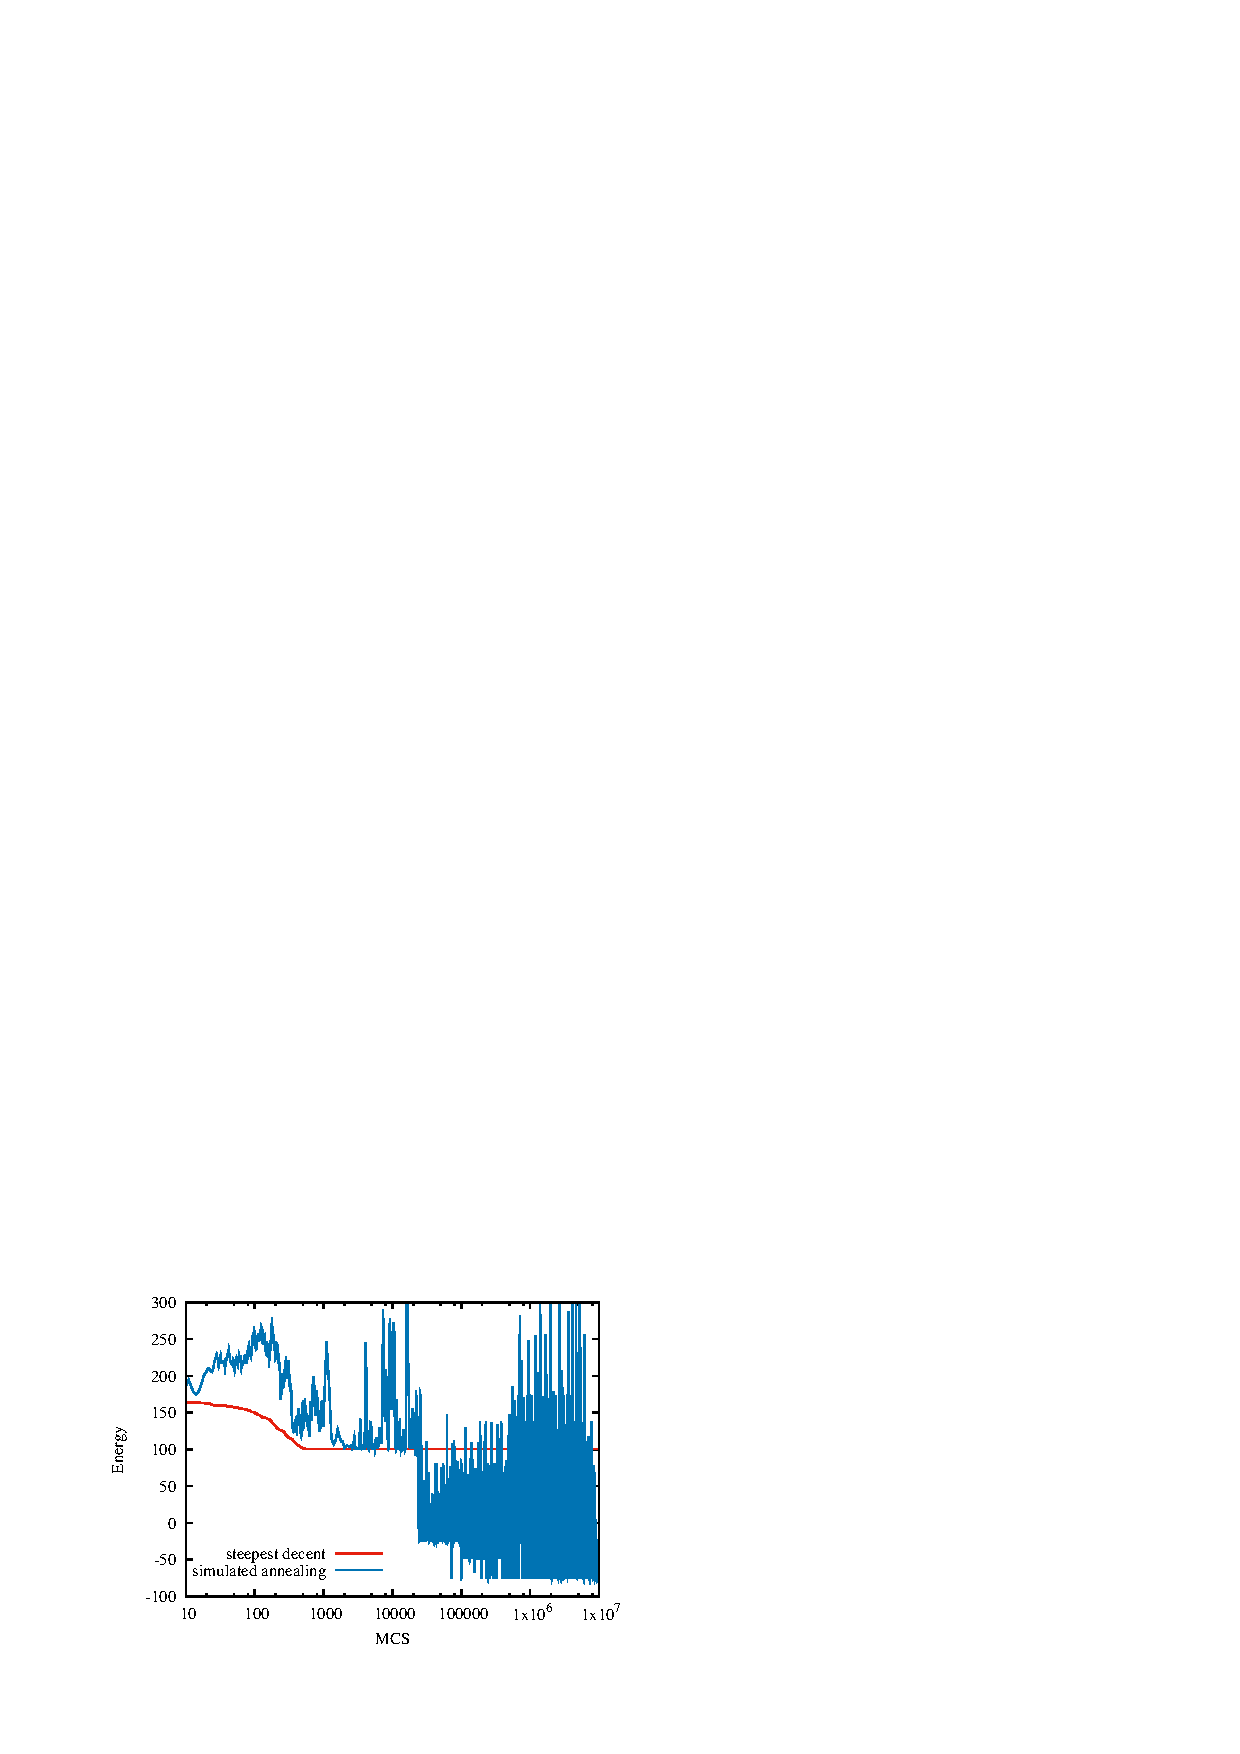
\includegraphics{image/energy.pdf}}

  \hspace*{17em}$T(t) = 100 - \frac{99}{10^7} t$
\end{frame}

\begin{frame}[t,fragile]{離散最適化問題への応用}
  \begin{itemize}
    \setlength{\itemsep}{1em}
  \item 微分を必要としないので、離散最適化問題にも適用可
    \begin{itemize}
    \item 例: 巡回セールスマン問題、数独、ナップザック問題
    \end{itemize}
  \item いかに状態とエネルギーを定義するかが重要
    \begin{itemize}
    \item 例: $n \times n$魔法陣 (行・列・ななめの和$M = n(n^2+1)/2$)
    \item 「状態」C: $1\sim n^2$の自然数をある順序でます目に並べたもの
    \item 「エネルギー」
      \[
      E(C) = \sum_{\rm row} (S_r-M)^2 + \sum_{\rm col} (S_c-M)^2 + \sum_{\rm diag} (S_d-M)^2
      \]
    \item 「正しい」魔方陣: $E(C) = 0$
    \end{itemize}
  \item 解の数(絶対零度のエントロピー)を求めるのにも利用できる
  \end{itemize}
\end{frame}


% -*- coding: utf-8 -*-

\section{最適化手法の比較}

\begin{frame}[t,fragile]{例題 (二次元の最適化)}
  \begin{center}
    \resizebox{.9\textwidth}{!}{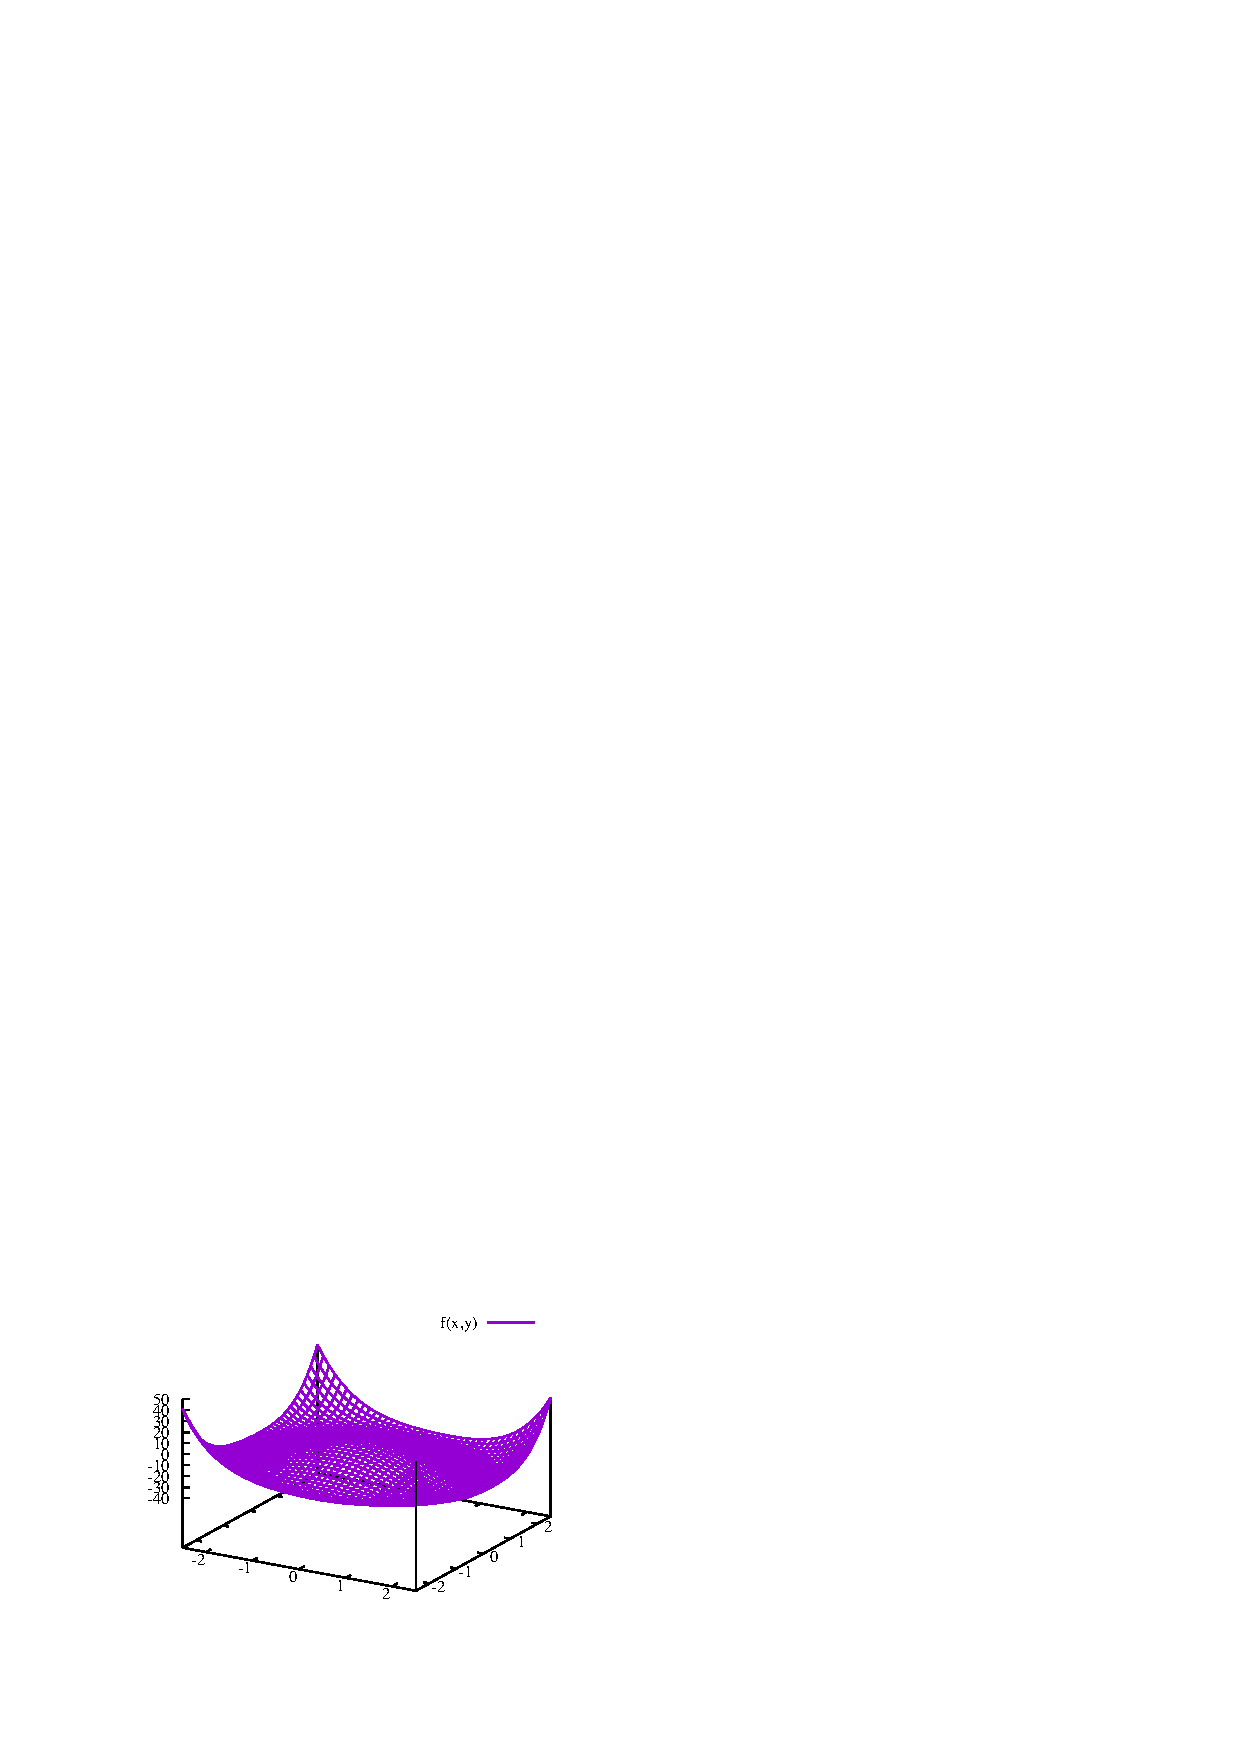
\includegraphics{image/func_2d.pdf}}
  \end{center}
\end{frame}

\begin{frame}[t,fragile]{様々な最適化手法の比較 (1/4)}
  \begin{center}
    \resizebox{.9\textwidth}{!}{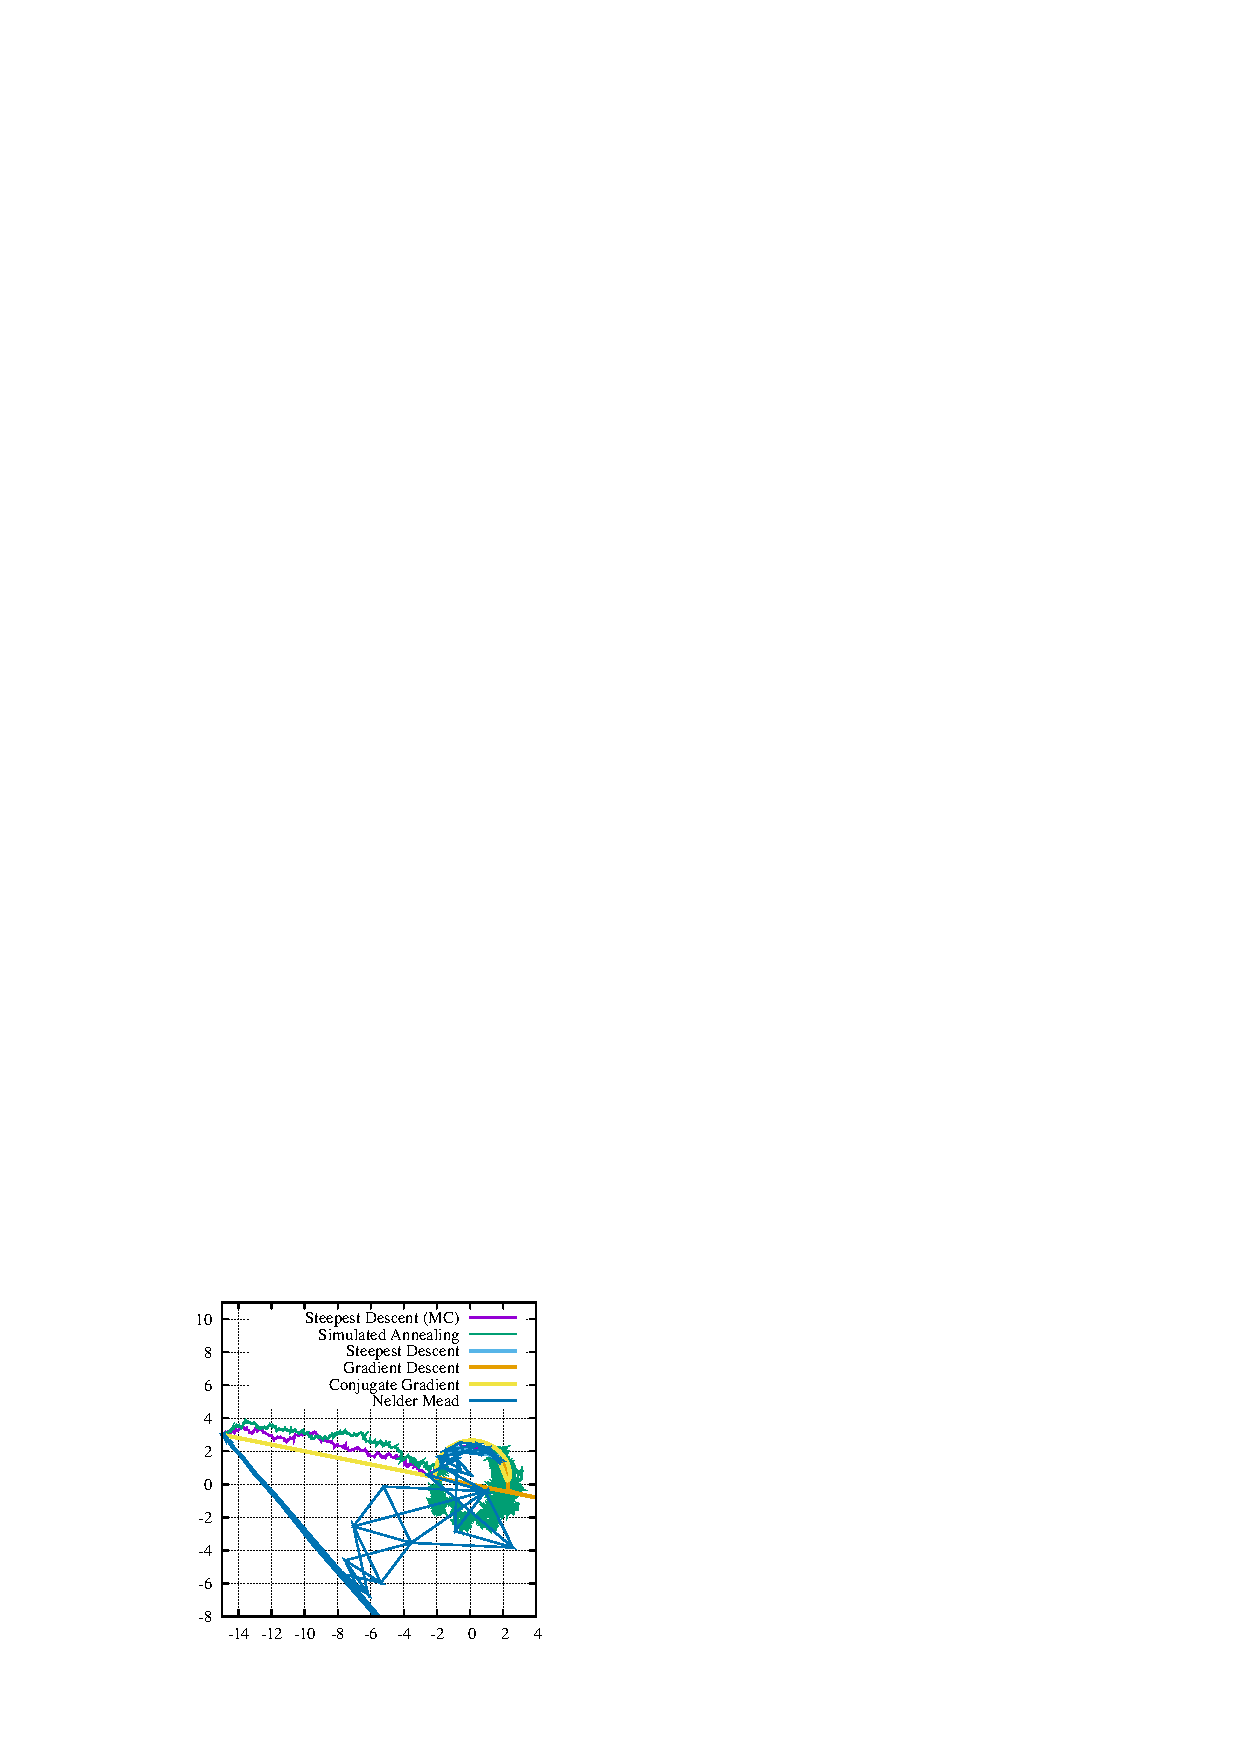
\includegraphics{image/optimization.pdf}}
  \end{center}
\end{frame}

\begin{frame}[t,fragile]{様々な最適化手法の比較 (2/4)}
  \begin{center}
    \resizebox{.9\textwidth}{!}{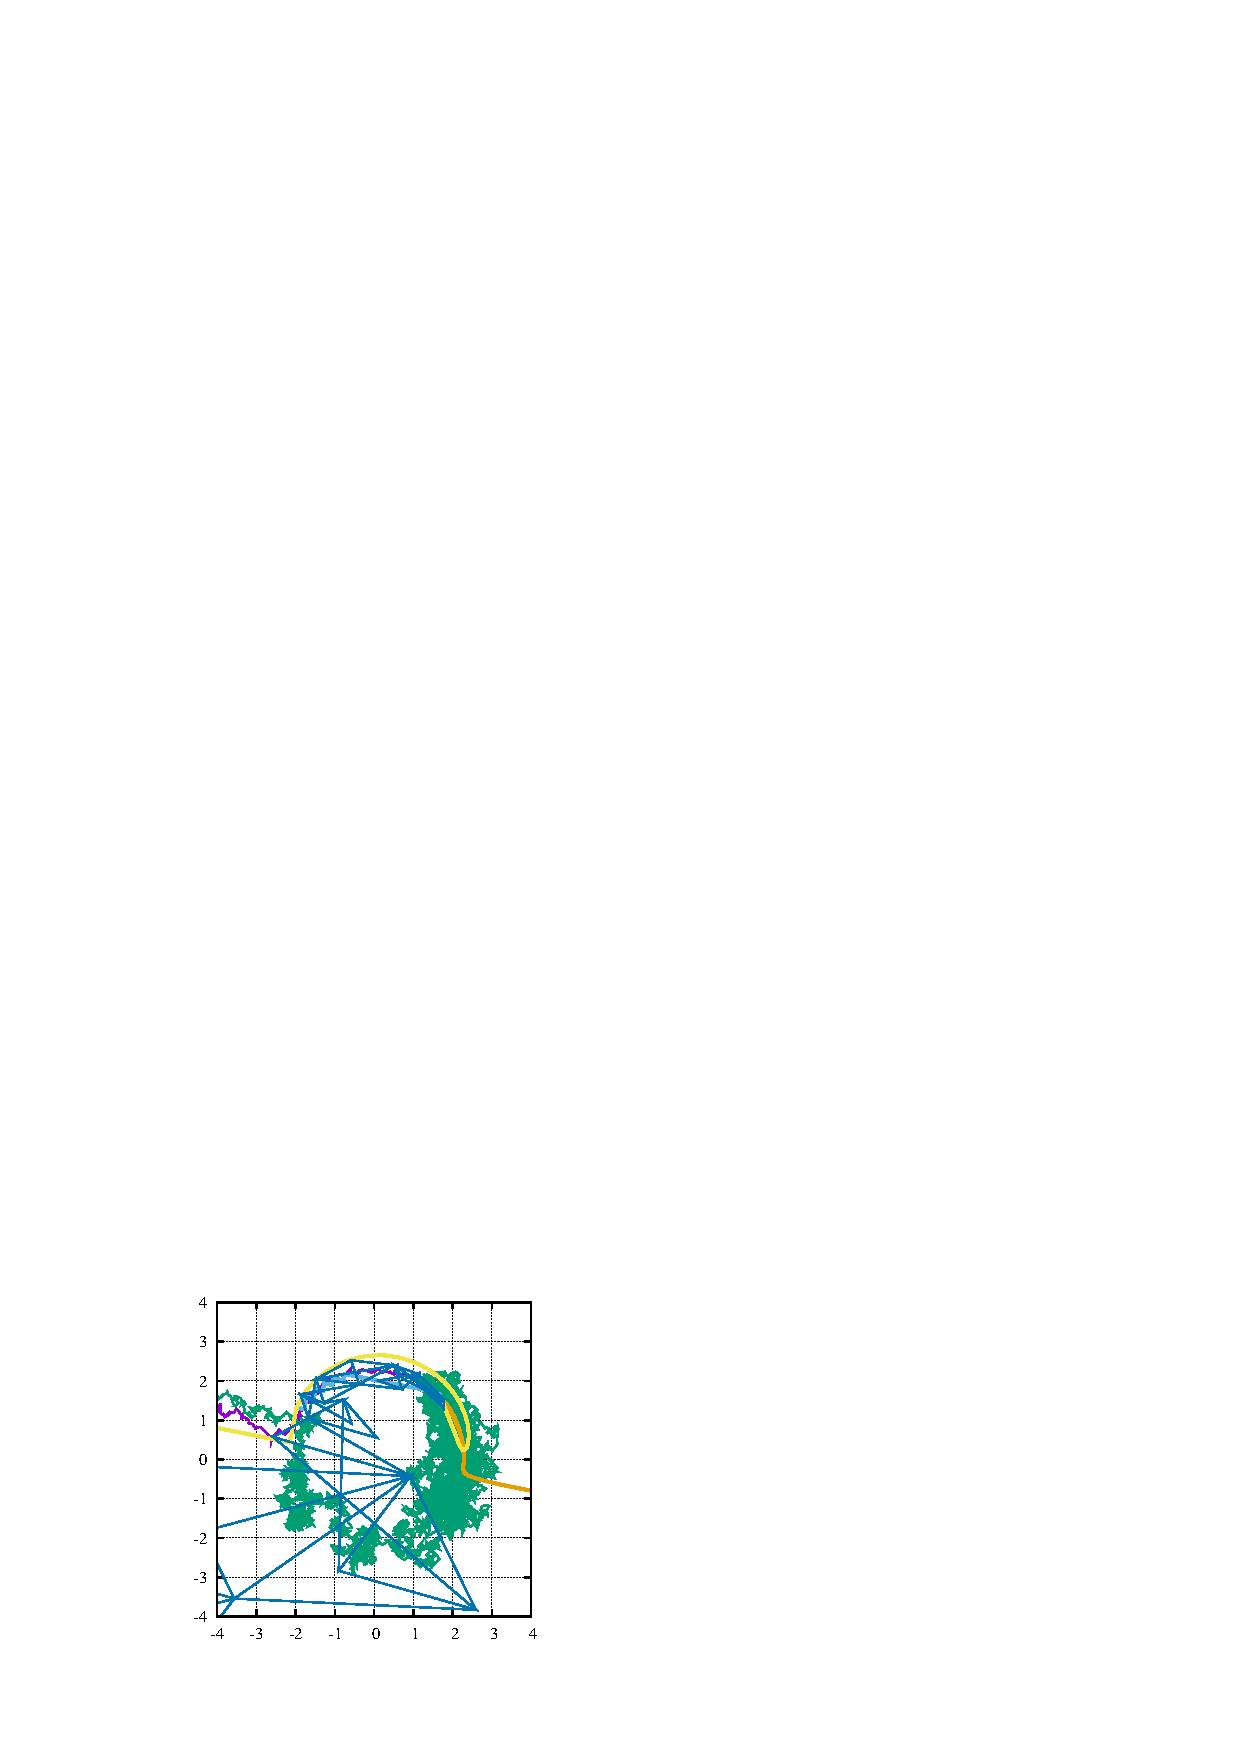
\includegraphics{image/optimization2.pdf}}
  \end{center}
\end{frame}

\begin{frame}[t,fragile]{様々な最適化手法の比較 (3/4)}
  \begin{center}
    \resizebox{.9\textwidth}{!}{\includegraphics{image/optimization3.pdf}}
  \end{center}
\end{frame}

\begin{frame}[t,fragile]{様々な最適化手法の比較 (4/4)}
  \begin{center}
    \resizebox{.9\textwidth}{!}{\includegraphics{image/optimization4.pdf}}
  \end{center}
\end{frame}

\begin{frame}[t,fragile]{真の解への近づき方}
  \begin{center}
    \resizebox{.9\textwidth}{!}{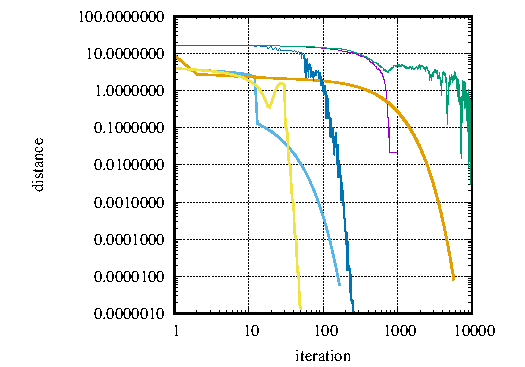
\includegraphics{image/convergence.pdf}}
  \end{center}
\end{frame}



\end{document}
